\documentclass[11pt]{article}
\usepackage[margin=1in]{geometry}
\usepackage{amsmath,amssymb,booktabs,graphicx,enumitem,caption}
\usepackage[hidelinks]{hyperref}
\captionsetup{font=small,labelfont=bf,skip=4pt}
\setlist[enumerate,1]{leftmargin=*,itemsep=6pt,label=\textbf{\arabic*.}}
\setlist[enumerate,2]{label=(\alph*),leftmargin=*,itemsep=4pt,topsep=3pt}
\setlength{\abovedisplayskip}{6pt}\setlength{\belowdisplayskip}{6pt}
\setlength{\abovedisplayshortskip}{4pt}\setlength{\belowdisplayshortskip}{4pt}
\renewcommand{\arraystretch}{1.1}
\renewcommand{\topfraction}{0.92}\renewcommand{\bottomfraction}{0.80}
\renewcommand{\textfraction}{0.08}\renewcommand{\floatpagefraction}{0.80}
\setcounter{topnumber}{3}\setcounter{bottomnumber}{2}\setcounter{totalnumber}{4}
\newcommand{\lhat}{\hat{\lambda}}

\begin{document}

\noindent Orlando Leng \hfill Homework 4
\vspace{2pt}\hrule\vspace{6pt}
\noindent\small Code, figures, and reproducible output:
\href{https://github.com/Orlandoxinchen/homework4-power-analysis}%
{\texttt{github.com/Orlandoxinchen/homework4-power-analysis}}\normalsize
\vspace{4pt}\hrule\vspace{12pt}

\begin{center}\large\textbf{Part 1.\quad Analytical Problems}\end{center}

\begin{enumerate}

%================================================== 1
\item \textbf{Normal Distribution and Standardization.}
$X\sim N(\mu=0.8\%,\ \sigma=2.5\%)$; standardize with $z=(x-\mu)/\sigma$.

\begin{enumerate}
\item $\displaystyle z=\frac{0-0.8}{2.5}=-0.32$, so
\[ P(X<0)=\Phi(-0.32)=\mathbf{0.3745}\quad(37.45\%). \]
Returns are negative on roughly 37 days in 100.

\item $\displaystyle z_1=\frac{-1-0.8}{2.5}=-0.72,\qquad z_2=\frac{3-0.8}{2.5}=0.88$, so
\[ P(-1\%<X<3\%)=\Phi(0.88)-\Phi(-0.72)=0.8106-0.2358=\mathbf{0.5748}\quad(57.48\%). \]

\item $\displaystyle z=\frac{4-0.8}{2.5}=1.28$, so
\[ P(X>4\%)=1-\Phi(1.28)=\mathbf{0.1003}\quad(\textbf{10.03\%\ of days}). \]

\item The 10th percentile of the standard normal is $z_{0.10}=-1.2816$, so
\[ x=\mu+z_{0.10}\,\sigma=0.8+(-1.2816)(2.5)=\mathbf{-2.404\%}. \]
The worst 10\% of days lose more than $2.40\%$.
\end{enumerate}

\begin{figure}[htbp]\centering
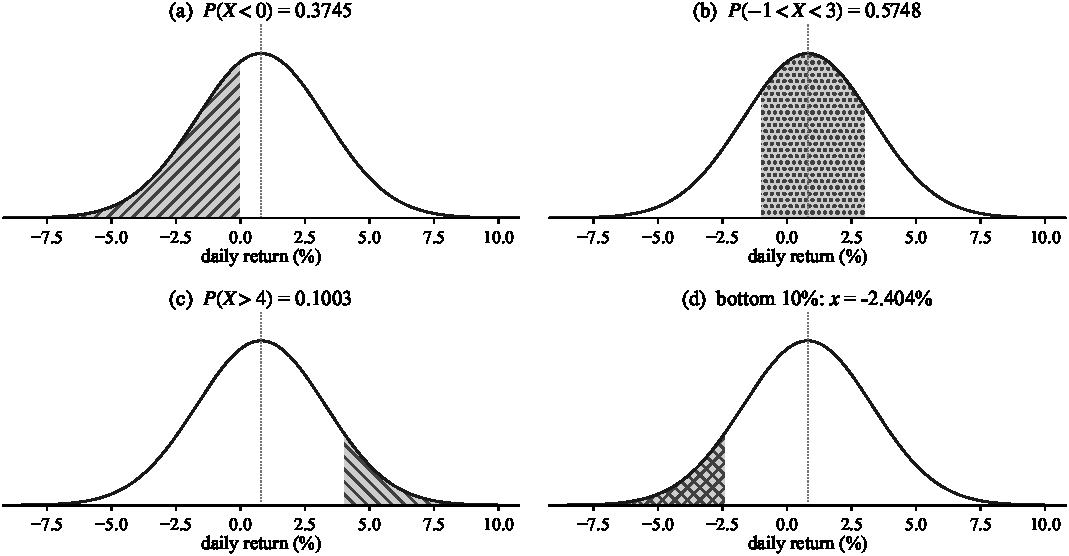
\includegraphics[width=\linewidth]{figures/p1_normal}
\caption{The four questions as areas under $N(0.8,2.5^2)$. The dotted line marks the mean.}
\end{figure}

%================================================== 2
\item \textbf{Maximum Likelihood Estimation.}
Data: $1.2,\,0.8,\,1.5,\,2.1,\,0.9,\,1.7,\,1.3,\,1.1,\,1.6,\,1.4$ seconds, so $n=10$ and
$\sum_{i=1}^{10}x_i=13.6$ (mean $\bar x=1.36$). Model: $f(x\mid\lambda)=\lambda e^{-\lambda x}$,
$x\ge0$, $\lambda>0$.

\begin{enumerate}
\item The observations are independent, so the likelihood is the product of the densities:
\[ L(\lambda\mid x_1,\dots,x_{10})=\prod_{i=1}^{10}\lambda e^{-\lambda x_i}
   =\lambda^{10}\exp\!\Big(-\lambda\sum_{i=1}^{10}x_i\Big)=\lambda^{10}e^{-13.6\lambda}. \]

\item Taking logs turns the product into a sum:
\[ \ell(\lambda)=\ln L(\lambda)=10\ln\lambda-\lambda\sum_{i=1}^{10}x_i=10\ln\lambda-13.6\lambda. \]

\item Differentiate, set to zero, and solve:
\[ \frac{d\ell}{d\lambda}=\frac{10}{\lambda}-13.6=0
   \quad\Longrightarrow\quad \lhat=\frac{10}{13.6}
   \qquad\text{in general}\quad \lhat=\frac{n}{\sum x_i}=\frac{1}{\bar x}. \]
This is a maximum, not a minimum, because
\[ \frac{d^2\ell}{d\lambda^2}=-\frac{10}{\lambda^2}<0 \quad\text{for every }\lambda>0, \]
so $\ell$ is strictly concave and the stationary point is the unique global maximum.

\item $\displaystyle \lhat=\frac{10}{13.6}=\mathbf{0.7353}$ requests per second. Equivalently the
fitted mean response time is $1/\lhat=\bar x=1.36$ seconds, which is the sanity check: the
exponential MLE just inverts the sample mean.
\end{enumerate}

\begin{figure}[htbp]\centering
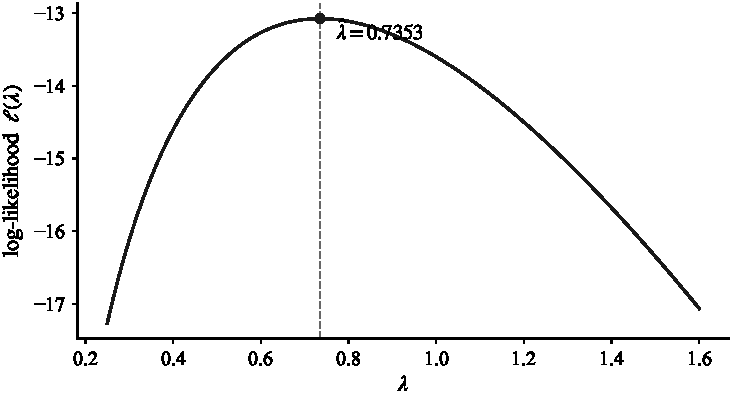
\includegraphics[width=0.60\linewidth]{figures/p2_loglik}
\caption{Log-likelihood $\ell(\lambda)=10\ln\lambda-13.6\lambda$, maximized at $\lhat=0.7353$.}
\end{figure}

%================================================== 3
\item \textbf{Power Analysis and Sample Size.} $p_0=0.08$, $\alpha=0.05$ one-tailed,
power $=0.80$, equal groups.

\begin{enumerate}
\item With $p_0$ the current rate and $p_1$ the redesign's rate,
\[ H_0:\ p_1=p_0=0.08 \qquad\text{(the redesign does not raise conversion)} \]
\[ H_1:\ p_1>0.08 \qquad\text{(the redesign raises conversion)} \]
one-tailed, because the question asks only whether the new design \emph{increases} conversion.

\item Power $=0.80$ means: \emph{if} the redesign truly lifts conversion from 8\% to 10\%, then an
experiment of this size will produce a significant result --- correctly rejecting $H_0$ --- in
80\% of repetitions. The complement is the Type II error rate, $\beta=0.20$: one time in five we
would run the test on a genuinely better design and still fail to detect it. Note that power is a
statement about what happens \emph{when $H_1$ is true}; it says nothing about the 5\% false-positive
rate, which is governed by $\alpha$.

\item With $z_{0.05}=1.645$, $z_{0.20}=0.84$, $p_0=0.08$, $p_1=0.10$:
\[ n=\frac{(z_\alpha+z_\beta)^2\big[p_0(1-p_0)+p_1(1-p_1)\big]}{(p_1-p_0)^2}
    =\frac{(2.485)^2\big[(0.08)(0.92)+(0.10)(0.90)\big]}{(0.02)^2} \]
\[ =\frac{6.175225\times(0.0736+0.0900)}{0.0004}
  =\frac{6.175225\times0.1636}{0.0004}=2525.67 \]
so $\mathbf{n=2{,}526}$ per group (5,052 visitors in total).

\item Same formula with $p_1=0.09$:
\[ n=\frac{6.175225\times\big[(0.08)(0.92)+(0.09)(0.91)\big]}{(0.01)^2}
  =\frac{6.175225\times(0.0736+0.0819)}{0.0001} \]
\[ =\frac{6.175225\times0.1555}{0.0001}=9602.47 \]
so $\mathbf{n=9{,}603}$ per group (19,206 in total).

\begin{figure}[htbp]\centering
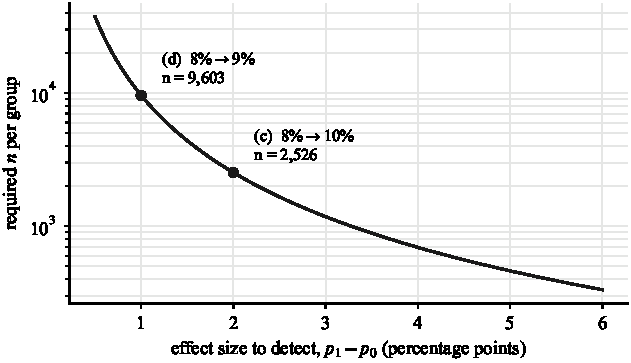
\includegraphics[width=0.62\linewidth]{figures/p3_samplesize}
\caption{Required sample size per group against the effect to be detected (log scale),
$\alpha=0.05$ one-tailed, power $0.80$, $p_0=8\%$.}
\end{figure}

\item Halving the effect to be detected multiplied the required sample by $9{,}603/2{,}526=3.80$,
close to the factor of 4 implied by $n\propto1/(p_1-p_0)^2$. (It falls a little short of exactly 4
only because the variance term $p_0(1-p_0)+p_1(1-p_1)$ also shrinks slightly, from 0.1636 to
0.1555, when $p_1$ moves closer to $p_0$.)

Intuitively: what the test must do is separate two sampling distributions whose centres are
$p_1-p_0$ apart and whose spread is the standard error, of order $\sqrt{p(1-p)/n}$. When the gap is
cut in half, the distributions overlap far more, and the only lever available is to shrink the
standard error until the gap is again several standard errors wide. But the standard error falls
only as $1/\sqrt{n}$, so halving it costs four times the data. Small effects are not slightly
harder to detect than large ones --- they are quadratically harder.
\end{enumerate}

\end{enumerate}

\clearpage
\begin{center}\large\textbf{Part 2.\quad Hypothesis Testing Simulation and Power Analysis}\end{center}

\noindent\small The full script is \texttt{hw4\_part2\_simulation.py} in the repository linked above;
\texttt{np.random.seed(42)} makes every number below reproducible.\normalsize
\vspace{8pt}

\noindent\textbf{Part A \quad Simulating the Type I error rate}

\smallskip
\noindent $H_0:\mu=50$ against $H_1:\mu\neq50$, with $\sigma=10$, $n=30$, $\alpha=0.05$, and 10,000
simulated samples drawn \emph{from the null distribution} $N(50,10^2)$. For each sample I compute
$\bar x$, then $z=(\bar x-50)/(\sigma/\sqrt n)$, then the two-sided $p$-value $2[1-\Phi(|z|)]$, and
reject when $p<\alpha$.

\begin{center}\small
\begin{tabular}{lr}
\toprule
Rejections & 548 of 10,000\\
Empirical Type I error rate & \textbf{0.0548}\\
Theoretical $\alpha$ & 0.0500\\
Monte Carlo standard error & 0.0022\\
\bottomrule
\end{tabular}
\end{center}

\begin{enumerate}[label=\textbf{(\alph*)},leftmargin=*,itemsep=4pt]
\item \textbf{Yes.} 0.0548 against a target of 0.0500 --- a gap of 0.0048, or about half a
percentage point.

\item \textbf{Because the rate is itself an estimate.} The number of rejections is
$\text{Binomial}(10{,}000,\,0.05)$, so the simulated rate has standard error
$\sqrt{0.05(0.95)/10{,}000}=0.0022$; roughly 95\% of runs land in $[0.046,0.054]$. This particular
run sits about $2.2$ standard errors high, which is on the high side but unremarkable. To confirm
that this is sampling noise and not a flaw in the procedure, I reran the same code with 40
different seeds: the average rate was $0.05001$, and the spread across runs ($0.00196$) matched the
theoretical Monte Carlo standard error ($0.00218$) closely. The test is behaving exactly as it
should; one run simply came out on the high side.

\item \textbf{The estimate would tighten, not change.} Monte Carlo error falls as
$1/\sqrt{n_{\text{sim}}}$, so going from 10,000 to 100,000 shrinks the standard error by
$\sqrt{10}\approx3.16$, from $0.0022$ to about $0.0007$. Typical runs would land within roughly
$\pm0.0014$ of $0.05$. It would still never be \emph{exactly} 0.05 --- more simulations buy
precision, not exactness.
\end{enumerate}

\vspace{6pt}
\noindent\textbf{Part B \quad Type II error and statistical power}

\smallskip
\noindent The test is held fixed at $H_0:\mu=50$ versus $H_1:\mu>50$ (right-tailed,
$p=1-\Phi(z)$), but the data are now generated from the \emph{true} distribution $N(53,10^2)$. Since
$H_0$ is false, failing to reject it is a Type II error. 10,000 simulations per sample size.

\begin{center}\small
\begin{tabular}{rrrr}
\toprule
Sample size & $\beta$ & Power & Power (theoretical)\\
\midrule
30  & 0.5036 & 0.4964 & 0.4993\\
60  & 0.2471 & 0.7529 & 0.7514\\
120 & 0.0507 & 0.9493 & 0.9497\\
\bottomrule
\end{tabular}
\end{center}

\noindent Power $+\ \beta=1$ holds exactly in every row, since every simulation either rejects or
fails to reject. The simulated values track the closed-form power
$1-\Phi\!\big(z_\alpha-(\mu_1-\mu_0)/(\sigma/\sqrt n)\big)$ to within Monte Carlo error.

\begin{enumerate}[label=\textbf{(\alph*)},leftmargin=*,itemsep=4pt]
\item \textbf{$\beta$ falls} as $n$ grows: $0.504\to0.247\to0.051$. Quadrupling the sample from 30
to 120 cut the miss rate by a factor of ten.
\item \textbf{Power rises} correspondingly: $0.496\to0.753\to0.949$. At $n=30$ the test is barely
better than a coin flip at detecting a real three-point difference; at $n=120$ it almost never
misses it.
\item The decisive quantity is the standardized distance between the truth and the null,
\[ \delta=\frac{\mu_{\text{true}}-\mu_0}{\sigma/\sqrt n}=\frac{3}{10/\sqrt n}=0.3\sqrt n, \]
which grows with $\sqrt n$: $1.64$ at $n=30$, $2.32$ at $n=60$, $3.29$ at $n=120$. The critical
value stays at $1.645$ no matter the sample size, so as $\delta$ grows the whole distribution of
$z$ slides to the right of it and the rejection probability climbs. Put plainly: a larger sample
makes $\bar x$ a steadier estimate, so a real three-point gap stops being something random noise
could plausibly have produced.
\end{enumerate}

\begin{figure}[htbp]\centering
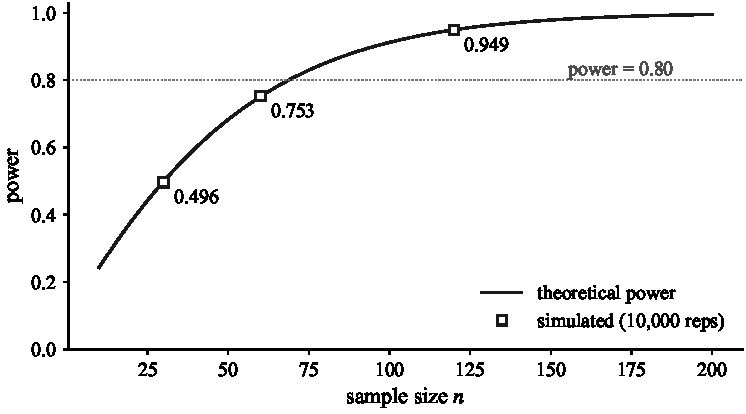
\includegraphics[width=0.74\linewidth]{figures/p2b_power_vs_n}
\caption{Power against sample size for $\mu_{\text{true}}=53$, $H_1:\mu>50$, $\alpha=0.05$.
Markers are the three simulated values; the curve is the closed-form power. Reaching the
conventional 0.80 target needs about $n=69$.}
\end{figure}

\vspace{6pt}
\noindent\textbf{Part C \quad Power curve}

\smallskip
\noindent Now the null is held at $\mu_0=50$ (two-sided, $\alpha=0.05$, $n=30$) while the
\emph{true} mean is swept over 51 values from 45 to 55, with 2,000 simulations at each.

\begin{figure}[htbp]\centering
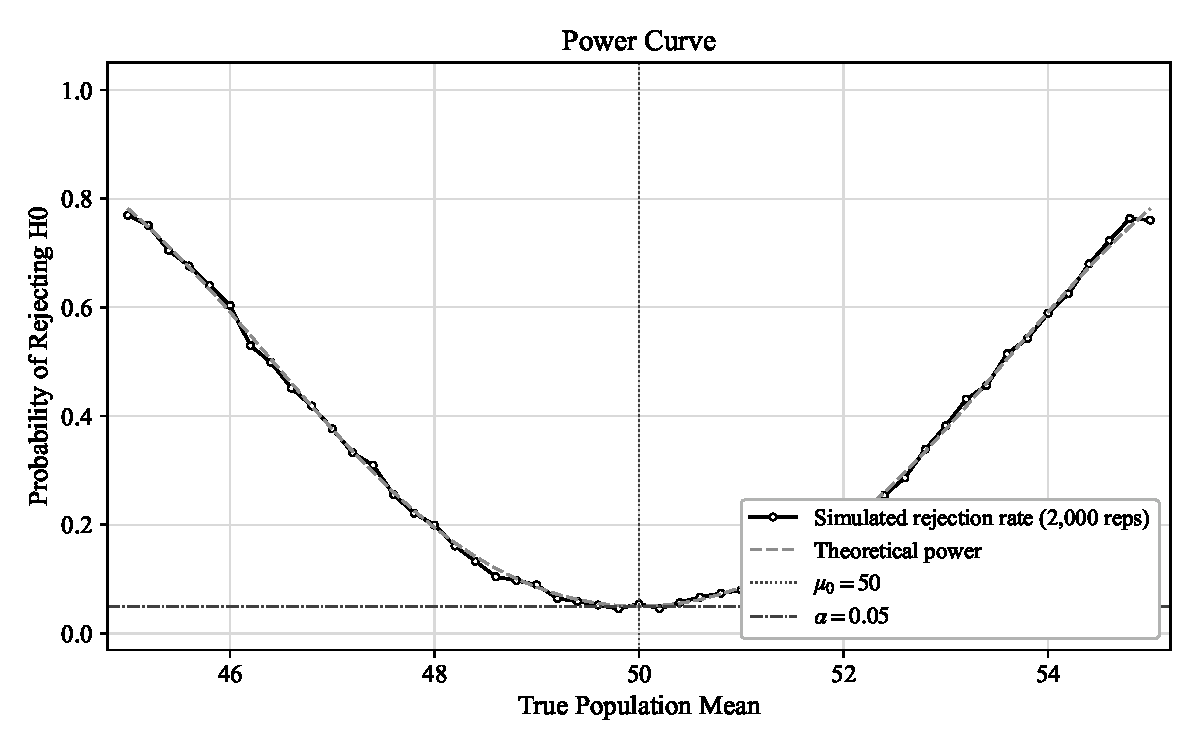
\includegraphics[width=\linewidth]{figures/power_curve}
\caption{Simulated rejection probability against the true population mean, with the closed-form
power curve for comparison.}
\end{figure}

\begin{enumerate}[label=\textbf{(\alph*)},leftmargin=*,itemsep=4pt]
\item \textbf{0.0545, which is $\alpha$.} When $\mu_{\text{true}}=50$ the null hypothesis is true,
so every rejection is a false positive. By construction the test rejects a true null with
probability $\alpha=0.05$, and the simulation recovers it. This single point on the curve is not
power at all --- it is the Type I error rate, which is why the curve bottoms out at $0.05$ rather
than at zero.

\item \textbf{Power rises toward 1} as the true mean moves away from 50 in either direction,
because the standardized distance $\delta=(\mu-50)/(\sigma/\sqrt n)$ grows and pushes the
distribution of $z$ past the critical values. At $\mu=53$ power is $0.38$; at $\mu=45$ or $55$ it
is about $0.77$.

\item \textbf{Symmetric because the test is two-sided and the normal is symmetric.} Power depends
on the true mean only through $|\delta|$, and the rejection region $|z|>1.96$ is itself symmetric
about $\mu_0$. So a true mean of 53 and a true mean of 47 are equally easy to detect --- the
simulation gives $0.382$ and $0.377$, differing only by Monte Carlo noise. A one-sided test would
break this symmetry immediately.

\item \textbf{The curve would become a much narrower, steeper well.} Power depends on $n$ only
through $\delta\propto\sqrt n$, so raising $n$ from 30 to 100 multiplies the standardized distance
by $\sqrt{100/30}=1.83$ at every true mean. The floor does not move --- the rejection rate at
$\mu=50$ stays at $\alpha=0.05$, since the Type I error rate is set by $\alpha$ and is unaffected by
sample size --- but the walls climb far more sharply:

\begin{center}\small
\begin{tabular}{rrr}
\toprule
True $\mu$ & Power, $n=30$ & Power, $n=100$\\
\midrule
50 & 0.0500 & 0.0500\\
51 & 0.0850 & 0.1701\\
52 & 0.1948 & 0.5160\\
53 & 0.3759 & 0.8508\\
54 & 0.5913 & 0.9793\\
\bottomrule
\end{tabular}
\end{center}
\end{enumerate}

\begin{figure}[t]\centering
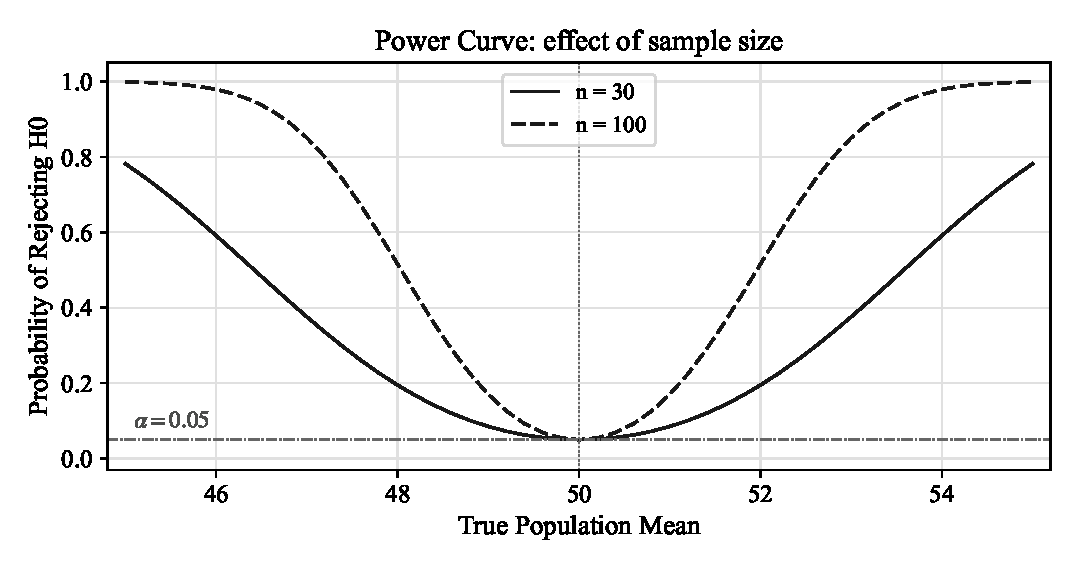
\includegraphics[width=0.80\linewidth]{figures/power_curve_n_comparison}
\caption{Effect of sample size on the power curve. The minimum stays pinned at $\alpha=0.05$;
only the steepness changes.}
\end{figure}

\end{document}
